\chapter{Diseño e Implementación}

En este capítulo mostraremos los detalles del diseño y la implementacion de diferentes partes del juego.

\section{Gramáticas y frases}

La parte de la generación automática de frases y definición de gramáticas es la más relevante del proyecto y la que la diferencia del resto de juegos de similares caracteríticas. Por ello consideramos esencial mostrar su funcionamiento.

\begin{figure}
    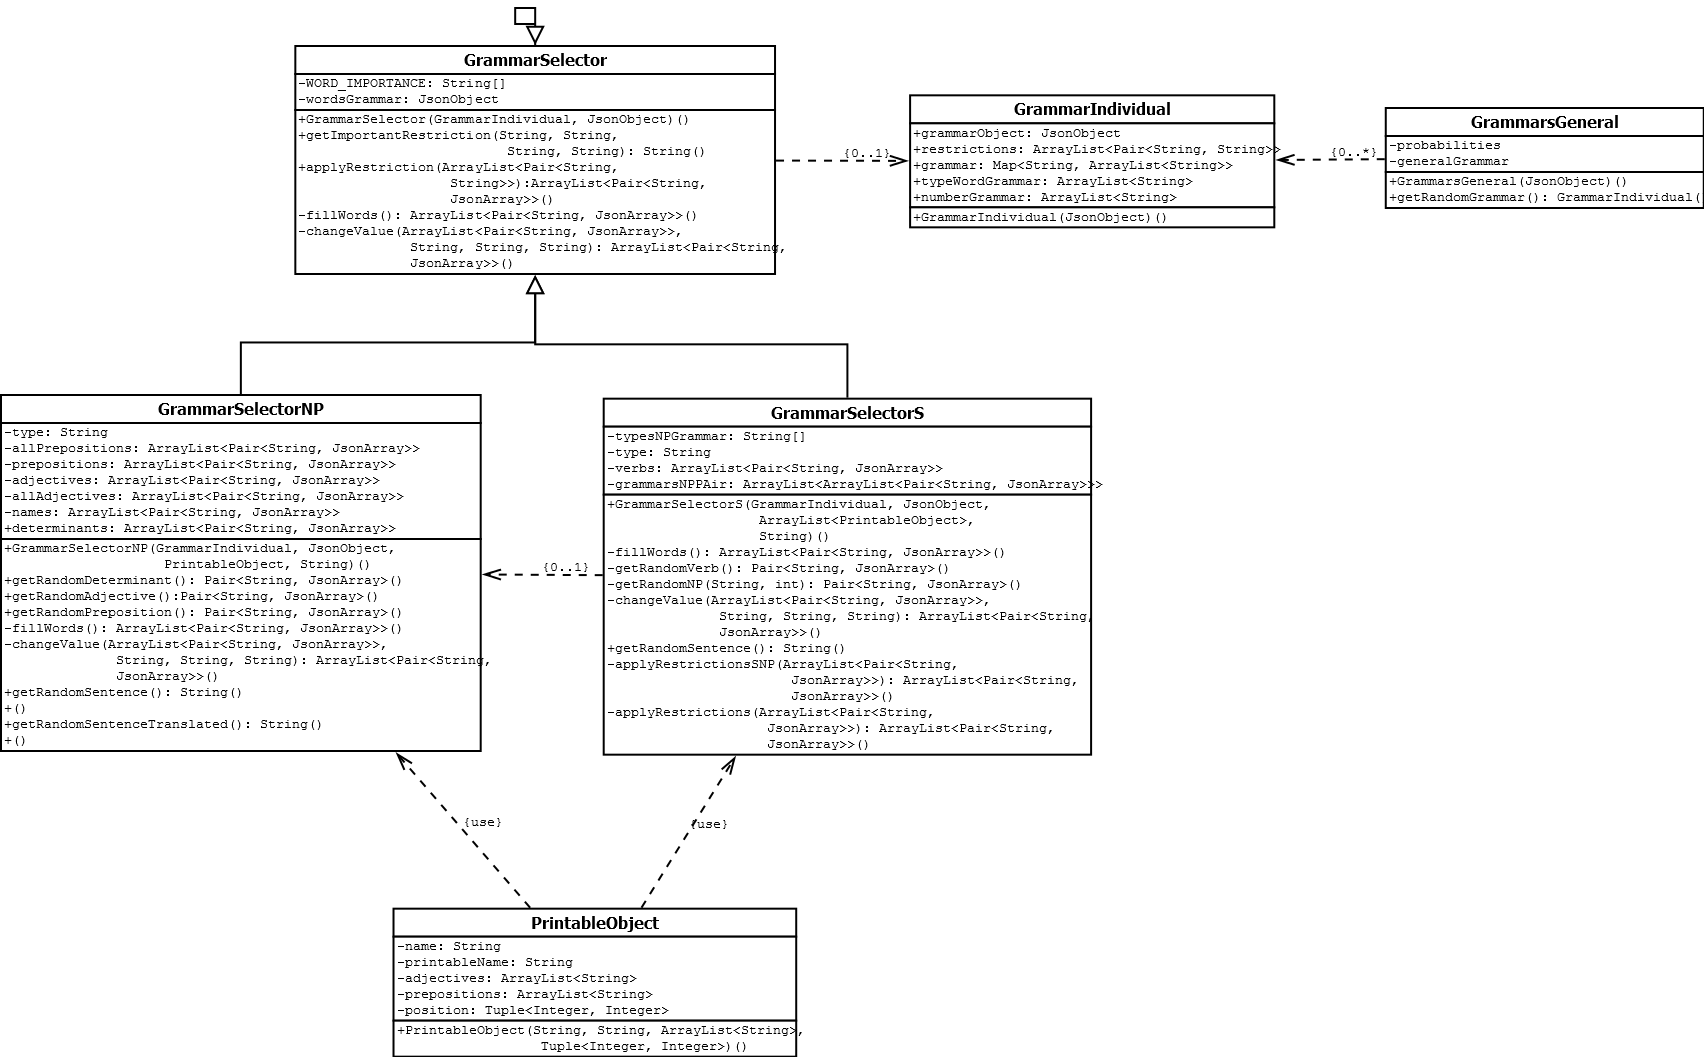
\includegraphics[width=\textwidth,height=\textheight,keepaspectratio,angle=90]{./img/grammarDiagram.png}
  \caption{Diagrama de clases de las gramáticas}
  \label{fig:clasesgramaticas}
\end{figure}

Tal y como se muestra en la figura ~\ref{clasesgramaticas}, la parte esencial de esta sección consta de seis clases, cuyo funcionamiento detallarremos a continuación.

\subsection{Explicación general del funcionamiento}

Tenemos dos clases (GrammarSelectorS y GrammarSelectorNP) que se encargan de generar las frases de manera aleatoria en base al nombre o nombres sobre los que queremos obtener dicha frase. La clase GrammarSelectorNP crea sintagmas nominales mientras que GrammarSelectorS crea frases usando dichos sintagmas nominales. Ambas usan diccionarios y gramáticas en un idioma en concreto especificado en el archivo de configuración \textit{language.properties}:

\begin{verbatim}
language=EN
\end{verbatim}

Parte de la dificultad de generar estas frases está en que todos los elementos de la misma deben de coincidir en base a las restricciones del propio idioma. Por ejemplo, los nombres, verbos y determinantes de una frase en español deben de coincidir en género y número. Este tipo de restricciones vienen dadas en las gramáticas que están especificadas en archivos JSON y que se comentarán más adelante.

Una vez detectemos que dos de las palabras no coinciden, cambiaremos la que tenga menor relevancia por la contraria dependiendo del tipo que sea (género o número):

\begin{lstlisting}[language=java]

if (toChange.equals(value1)) {
    changeToValue = JSONParsing.getElement(restrictions1, type + "opposite");
    typeChangeToValue = typeFirstRestriction; 
     
} else {
    changeToValue = JSONParsing.getElement(restrictions2, type + "opposite");
    typeChangeToValue = typeSecondRestriction;
}
this.changeValue(sentenceArray, toChange, changeToValue, typeChangeToValue);

\end{lstlisting}

De esta manera, siempre que haya una discordancia entre algunas de las palabras de una frase, iteraremos entre toda ella buscando una solución hasta que sea coherente, cambiando las palabras menos relevantes dentro de dicha frase para que se adapten al resto.

La clase GeneralGrammar, por su parte, obtiene la información de varias gramáticas (que es como vienen dadas en el fichero, dado que para describir una misma situación puede haber varias gramáticas que funcionen de la misma manera) y dispone de una función que devuelve una gramática individual (de la clase GrammarIndividual), que es la que usaremos a la hora de generar la frase en sí. Es decir, cuando queremos generar una frase de una gramática en concreto (por ejemplo cuando un personaje ataca a otro), seleccionaremos una de estas gramáticas al azar de todas las que estén disponibles en el idioma que tenemos (esto lo realiza la clase GrammarsGeneral) y luego usamos esa gramática en particular con GrammarIndividual.  De esta forma no siempre usamos la misma gramática y dependerá de la seleccionada aleatoriamente en GrammarsGeneral.

La clase PrintableObject es una superclase abstracta de la que heredan todos los objetos que pueden ser representados en el juego. Esta clase se encarga de obligar que dichos objetos tengan ciertas variables como el nombre o la capacidad de traducir su nombre a diferentes idiomas, así como una función que devuelve la posición en la que se encuentra en base al usuario (usado a la hora de describir lo que hay alrededor de un personaje).

Cabe destacar que estas gramáticas, al igual que los diccionarios usados para cada uno de los idiomas, se obtienen en base a ficheros JSON dados.

\subsection{\textit{Input} de gramáticas y diccionario}

Tal y como hemos mencionado anteriormente, tanto las gramáticas como los diccionarios son archivos JSON que el usuario puede cambiar y que afectará al resultado de las frases generadas.

Para las gramáticas tenemos dos archivos por idioma (tres si también contamos el diccionario). Uno de ellos son las gramáticas con las que creamos sintagmas nominales, mientras que las otras creamos frases usando, en su mayor parte, estos sintagmas nominales.

\subsubsection{Gramáticas: Sintagmas nominales}

Ejemplo de gramáticas de sintagma nominal en inglés:

\begin{lstlisting}[style=json]
"DETADJN": {
    "GM_1": {
        "S": 
            [
            {"DET_1": ""}, 
            {"ADJ_1": ""}, 
            {"N_1": ""}
        ],
        "restrictions": [
            {"DET_1.num": "N_1.num"},
            {"N_1.num": "ADJ_1.num"}
        ]
    }
}
\end{lstlisting}

En estas gramáticas especificamos, primero, el nombre de la gramática (en este caso, DETADJN). Este nombre es usado por el programa y ayudará al usuario a entender el tipo de gramática o grupo de gramáticas que son.

El siguiente nombre es el nombre de la gramática en particular. No es usado en el programa, pero su uso es necesario para poder definir varias gramáticas sobre el mismo árbol (si queremos varias gramáticas de tipo DETADJN, necesitaremos que se especifiquen el nombre de cada una de ellas).

Luego viene el contenido relevante. Primero nos encontramos con \textit{S}, que es donde se almacenará la definición de la gramática en sí; y luego \textit{restrictions} que, como su nombre indica, es donde especificaremos las restricciones de dicha gramática.

En la parte de la gramática tenemos, en este caso, \textit{DET\_1}, que es el primer determinante (y único) de la gramática, \textit{ADJ\_1}, el primer y único adjetivo que tiene dicha gramática y \textit{N\_1}, que es el nombre o sustantivo.
En las restricciones detallaremos las partes de la gramática que tienen que coincidir. En esta gramática solamente tenemos que el determinante, nombre y adjetivo tienen que ser iguales en número. Es decir, que ``the red swords'' no sería generada, sino que generaría ``the red sword''.

Este es un ejemplo en inglés, cuyas restricciones son más sencillas que en otros idiomas como el español o el gallego, donde los nombres, determinantes y adjetivos no solamente tienen que coincidir número, pero también en género. Por este motivo, para generar el mismo tipo de gramática para estos idiomas necesitaremos hacer lo siguiente:

\begin{lstlisting}[style=json]
"DETADJN": {
    "GM_1": {
        "S": 
            [
            {"DET_1": ""},
            {"N_1": ""},
            {"ADJ_1": ""}
        ],
        "restrictions": [
            {"DET_1.num": "N_1.num"},
            {"N_1.num": "ADJ_1.num"},
            {"DET_1.gen": "N_1.gen"},
            {"N_1.gen": "ADJ_1.gen"}
        ]
    }
}
\end{lstlisting}

Nótese que no solamente hemos añadido el género a las restricciones (para que no podamos generar frases como ``la espada rojo'' o ``el espada roja''), pero también hemos cambiado el orden del nombre y adjetivo para que se adapten tanto en español como en gallego. 

A la hora de cambiar las palabras dispondremos de un array donde somos capaces de ordenar las palabras por importancia. Un sustantivo es más importante que un determinante, por lo que si una de las restricciones no se cumple por culpa de algunos de estos dos elementos, el determinante será en que cambiará para adaptarse al género y número del nombre.

De esta manera podremos adaptar gramáticas a idiomas diferentes de una forma muy fácil y sin necesidad de tocar nada de código.

\subsubsection{Gramáticas: Frases}

Las gramáticas para la generación de frases también usa aquellas de sintagma nominal: 

\begin{lstlisting}[style=json]
"ATTACK": {
	"S1": {
	    "S": [
	        {"DETADJN_1": ""},
	        {"V_1": ""},
	        {"DETADJN_2": ""},
	        {"SIMPLEPREP_1": ""}
	    ],
	    "restrictions": [
	        {"DETADJN_1.num": "V_1.num"}
	    ]
	},
	"S2": {
	    "S": [
	        {"GENERAL_1": ""},
	        {"V_1": ""},
	        {"SIMPLE_2": ""},
	        {"SIMPLEPREP_1": ""}
	    ],
	    "restrictions": [
	        {"GENERAL_1.num": "V_1.num"}
	    ]
	}
}
\end{lstlisting}

La estructura de esta gramática es idéntica a la mencionada anteriormente. En este caso vemos que dentro de ``ATTACK'' disponemos de dos gramáticas distintas (este es solamente un ejemplo, en el juego tenemos muchas más disponibles) y éstas llaman a sintagmas nominales como el anterior.
Con la primera gramática podríamos generar una frase del estilo ``The mighty dragon attacks the brave hero with the sword"". En este ejemplo cabe destacar que las restricciones se pueden definir, no solamente entre palabras, pero también entre sintagmas nominales (siempre y cuando sea en comparación con una palabra que pueda ser cambiante, en este caso el verbo) y que los sintagmas nominales que son creados dentro de esta gramática tienen sus propias restricciones, por lo que siempre serán generadas de manera correcta.

\subsubsection{Diccionarios}

Al igual que las gramáticas, los diccionarios también están divididos por idiomas y son archivos JSON. Éste es un ejemplo de parte de una gramática en inglés:

\begin{lstlisting}[style=json]
"DET": {
    "the": [
        {"num": ""},
        {"translation": "the"},
        {"numopposite": "the"},
        {"genopposite": ""}
        {"gender": ""}
    ]
},
\end{lstlisting}

El primer elemento, ``DET'', especifica el tipo de palabra que es (determinante). El siguiente elemento especifica la palabra en sí (``the''). El resto de elementos estarán en un array, aunque en este caso no importa el orden. El primer elemento en esta lista es ``num'', es decir, si el elemento es singular o plural (para esta palabra esta información es innecesaria, por eso es un string vacío) y en ``numopposite'' guardaremos la palabra en el número contrario (si la palabra es singular, entonces guardaremos la palabra en plural).
El segundo es ``translation''. Todas las palabras entre los diccionarios serán las mismas o, por lo menos, las que están definidas en inglés también deben de estar en otros idiomas. En este valor almacenaremos la traducción de esta palabra en el idioma del diccionario que estaremos definiendo.
``gender'' y ``genopposite'', al igual que con ``num'' y ``numopposite'', almacenan el género de la palabra y la palabra en el género contrario.

Con los determinantes en inglés no hay mucho cambio, pero en español sí que es bastante diferente:

\begin{lstlisting}[style=json]
"DET": {
        "the": [
            {"num": "sing"},
            {"translation": "el"},
            {"numopposite": "los"},
            {"genopposite": "la"},
            {"gen": "mas"}
        ],
        "la": [
            {"num": "sing"},
            {"translation": "la"},
            {"numopposite": "las"},
            {"genopposite": "the"},
            {"gen": "fem"}
        ],
        "los": [
            {"num": "plural"},
            {"translation": "los"},
            {"numopposite": "the"},
            {"genopposite": "las"},
            {"gen": "mas"}
        ],
        "las": [
            {"num": "plural"},
            {"translation": "las"},
            {"numopposite": "la"},
            {"genopposite": "los"},
            {"gen": "fem"}
        ]
    },
\end{lstlisting}

En este caso seguimos definiendo ``the'', dado que es la clave en inglés y la palabra que se tiene que mantener. Sí que vemos que ``numopposite'' y ``genopposite'' apuntan a ``la''y ``los'', que son las nuevas entradas de determinantes en español. De esta forma siempre obtendremos la palabra que queramos siempre y cuando el programa precise de obtener un tipo de palabra concreta en base a las restricciones que contenga la gramática.

\section{Otras partes del sistema}

Las gramáticas juegan un papel muy importante en el proyecto, pero hay otras partes también relevantes que requieren una atención especial. Aquí mencionamos unas pocas:

\subsection{Interfaz de usuario para el texto generado}

Los invidentes usan diferentes programas que leen el texto que se muestra en la pantalla. Para ello nuestro juego debe de mostrar texto de alguna forma y ser capaz de que el lector pueda leerlo, lo que no es del todo trivial dado que hay que tener en cuenta diferentes aspectos para que el lector lea lo que queramos y no otras partes que no nos interesan. Más información sobre este tema se encuentra en la sección de instalación ~\ref{ref:instalacion}.

\subsubsection{Primera idea: pop-up}

La forma más sencilla de mostrar este texto es generar un ``pop-up'' cada vez que una frase es generada. De esta forma el usuario se enterará inmediatamente de lo que está sucediendo y, en caso de que haya una persona vidente a su lado, ésta también podrá leer la frase que se ha generado. Además, la frase no desaparecerá hasta que se presione la tecla de intro o se haga click en \textit{Aceptar}, por lo que es muy sencillo reproducirla la cantidad de veces que se desee.

La imagen ~\ref{lastiterationui} muestra el aspecto de nuestro \textit{roguelike} con esta idea implementada.

\begin{figure}
    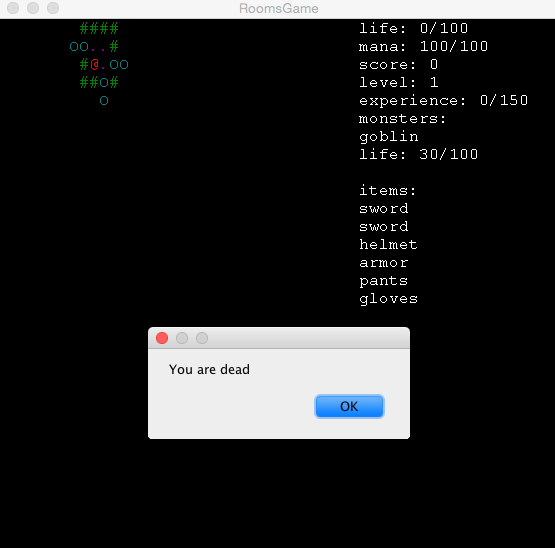
\includegraphics[width=\textwidth,height=\textheight,keepaspectratio]{./img/firstiterationui.png}
  \caption{Versión definitiva de la interfaz de usuario para el texto generado}
  \label{fig:firstiterationui}
\end{figure}

\subsubsection{Segunda idea: \textit{TextArea}}

Tras recibir el feedback decidimos cambiar la forma en la que mostramos al usuario estas frases por tres razones. La primera es que resulta desconcertante para el jugador vidente, dado que no es necesario para él o ella. Esto se podría solventar añadiendo una opción que se permita activar o desactivar esta opción, pero no es la mejor solución para este problema.
La segunda razón es que estos ``pop-ups'' no son un mecanismo de salida óptimo para las salidas rutinarias, como en nuestro caso, y rompe el ``flujo de trabajo''.
La tercera y última razón es que los usuarios invidentes no suelen usar elementos de este tipo, si no que están más acostumbrados a usar areas de texto donde se almacenan las últimas frases generadas.

En base a estas ideas decidimos crear un área de texto que permanecerá abierta siempre y cuando el jugador no decida cerrarla (permitiendo a los usuarios videntes no usarla). Una vez que algo suceda en el juego que requiera que se genere una descripción, dicha descripción será enviada al área de texto, el ``foco'' de las aplicaciones cambiará para que se sitúe en esa misma ventana y el lector de pantalla que usemos leerá dicha descripción. Mientras generemos frases el ``foco'' seguirá en esa área de texto (las teclas que pulsemos seguirán afectando al juego en sí). El foco solamente volverá al juego cuando pulsemos una tecla que no genere una nueva frase.
De esta forma solucionamos todos los inconvenientes que los ``pop-ups'' causaban a los usuarios y mejoramos la interfaz gráfica y accesibilidad del proyecto.

En ~\ref{lastiterationui} se puede encontrar una captura de pantalla donde se muestra el estado final de la parte de la interfaz de usuario que muestra las frases generadas.

\begin{figure}
    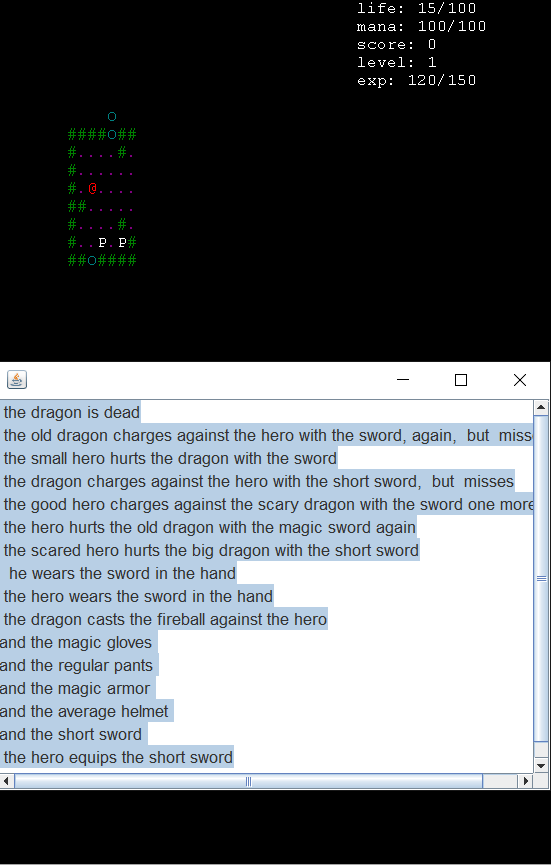
\includegraphics[width=\textwidth,height=\textheight,keepaspectratio]{./img/lastiterationui.png}
  \caption{Versión definitiva de la interfaz de usuario para el texto generado}
  \label{fig:lastiterationui}
\end{figure}

\subsection{Generación aleatoria de mapas y elementos}

La generación aleatoria de mapas y elementos dentro del mismo es muy importante en un juego de género \textit{roguelike}. A continuación explicaremos las decisiones tomadas en base a este tema.

\subsubsection{Primera idea: Generación completamente aleatoria}

En un primer momento nuestra decisión fue la de generar todo de manera aleatoria, sin considerar ningún aspecto externo, pero manteniendo la generalidad en el código para poder cambiar su comportamiento en cualquier momento. Esto causaba que algunas mazmorras fueran muy complicadas cuando el jugador todavía no tenía el equipamiento necesario para enfrentarse a dichos enemigos o demasiado sencilla en otros momentos.

Este problema fue mencionado la primera vez que recibimos \textit{feedback} y por ello decidimos cambiarlo por algo un poco más complejo. En el mundo del rol, tener en cuenta ciertas características del usuario para generar elementos externos se denomina \textit{generación de encuentros}.

\subsubsection{Segunda idea: Generador de encuentros}
\label{generadorencuentros}

En vez de generar mapas, enemigos y elementos de manera completamente aleatoria, podemos generarlos en base al nivel que tienen ciertos personajes. Si el personaje que controla el usuario tiene nivel 10, entonces los adversarios que se encuentran deben de ser de un nivel, por ejemplo, entre 8 y 12, mientras que los elementos que los oponentes sueltan al morir (como las espadas y armaduras) también deben de tener un nivel similar para que la progresión tenga sentido y eliminar enemigos tenga un cierto nivel de recompensa.

De esta forma podremos, en base al nivel dado, podremos generar contrincarios con diferentes características que se adapten a lo que necesitamos:

\begin{lstlisting}[language=java]
Rat rat = new Rat(this.getMap(), this, position, new ArrayList<String>(), level);
\end{lstlisting}

\subsection{Comportamiento de los enemigos}

Como cabe suponer, los adversarios que nos encontramos en el juego se moverán de diferentes formas, por lo que tendremos que diseñarlo de una manera genérica que nos permita realizar esto de la forma más simple posible.
Para ello nos hemos basado en el patrón de diseño \textit{estrategia} porque se adapta perfectamente a nuestros requisitos.

Los tipos de movimiento que tenemos en el juego actualmente son los siguientes:

\paragraph{RandomMovement:} Los enemigos son ``pasivos'', es decir, no atacarán a ningún personaje ni tampoco irán hacia él en ningún momento.

\paragraph{FollowingMovementDumb:} Los contrincantes que tengan este tipo de movimiento son ``agresivos''. Seguirán al jugador e intentarán atacarle, pero no se mueven de una forma óptima para lograr su meta, por lo que esquivarlos no suele ser muy complicado.

\paragraph{FollowingMovement:} Este tipo de movimiento es el más complejo. El enemigo se moverá de manera precisa para llegar lo antes posible al usuario y usará todo tipo de herramientas para derrotarlo (como el uso de magia o atacándole cuerpo a cuerpo).

Crear nuevos tipos de movimientos es una tarea trivial, ya que solamente tendríamos que implementar la interfaz \textit{Movement} con la única función que posee e insertar el código del nuevo tipo de movimiento en él.

En ~\ref{fig:iaenemy} mostramos el diagrama de clases que hemos implementado en nuestro sistema y que contiene el patrón de diseño \textit{estrategia}, tal y como hemos comentado.

\begin{figure}
    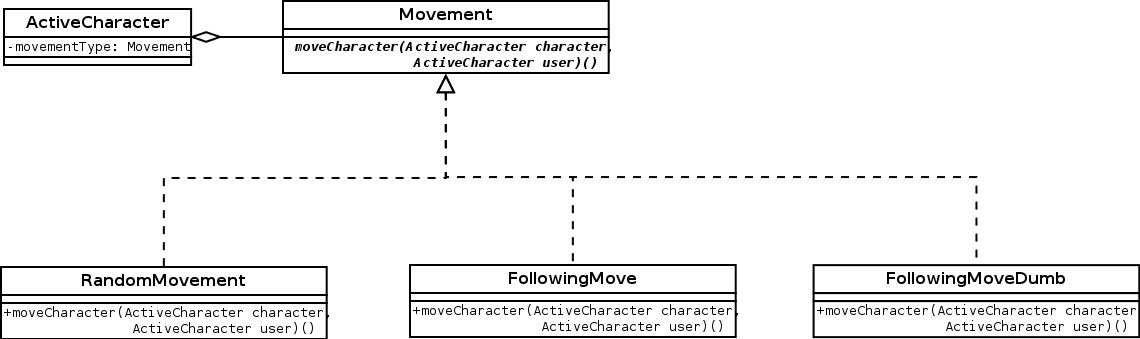
\includegraphics[width=\textwidth,height=\textheight,keepaspectratio]{./img/iaenemy.png}
  \caption{Diagrama de clases sobre el comportamiento de los enemigos}
  \label{fig:iaenemy}
\end{figure}

\section{Herramientas empleadas}

En esta sección hablaremos sobre las tecnologías empleadas en este proyecto y, si cabe, las razones por la que fueron elegidas. En primer lugar describiremos las herramientas y bibliotecas que hemos usado y, en segundo lugar, las herramientas de comunicación con usuarios y \textit{testers}.

\paragraph{Java:} Lenguaje de programación orientado a objetos cuya primera aparición fue en 1995. Es uno de los lenguajes de programación más utilizados en la industria y una de sus principales características es que es multiplataforma, es decir, puede ser ejecutado en cualquier sistema operativo que tenga la \textit{Java Virtual Machine} instalada sin necesidad de realizar cambios en el código (WORA, \textit{Write once, run anywhere}). Esta ventaja es primordial en nuestro caso, dado que nuestros usuarios potenciales usan una gran variedad de sistemas operativos.

 \paragraph{\href{https://eclipse.org}{Eclipse}:} Es un IDE (entorno de desarrollo integrado) usado para escribir código en múltiples idiomas. También incluye una serie de \textit{plugins} que facilitan y automatizan muchas de las labores a realizar como el uso de sistema de controles, ejecución de código y tests, herramientas de \textit{debug}, autocompletado de código, etc.

 \paragraph{\href{https://goo.gl/IKsKt5}{Git}:} Sistema de control de versiones distribuido introducido en 2005 y desarrollado principalmente por Linus Torvalds. Es el control de versiones referencia en la mayoría de empresas y proyectos de software libre gracias a su rapidez y, al ser distribuido, permite trabajar y realizar \textit{commits} del código sin necesidad de conexión a Internet.

 \paragraph{\href{github.com}{GitHub}:} Plataforma de desarrollo colaborativo usada para alojar proyectos usando el sistema de control de versiones Git. La mayoría de proyectos de código abierto lo usan, dado que es gratuito, aunque permite la opción de almacenar el código de forma privada previo pago.

\paragraph{JSON:} \textit{JavaScript Object Notation}. Es un formato muy usado en APIs para intercambio de datos, similar a XML. En nuestro caso lo usamos para definir las gramáticas y diccionarios de nuestro proyecto, dado que es muy sencillo de leer y especificar. Hay numerosas bibliotecas que nos permiten analizar y trabajar con este formato en Java. En nuestro caso hemos usado \href{https://goo.gl/zPCXen}{\textit{Gson}}.

\paragraph{\href{www.nvaccess.org}{\textit{NVDA}}:} Lector de pantalla de código libre para Windows que narra el tipo de ventanas y texto que se encuentran en la pantalla, facilitando el uso del ordenador y otros dispositivos a los usuarios invidentes. 
Orca es, en cierta medida, su equivalente en Linux. Otras alternativas son \href{https://goo.gl/GoghW7}{BrowseAloud} o \href{http://goo.gl/OAB7VC}{Microsoft Narrator}. Hemos elegido \textit{NVDA} por ser la alternativa libre más usada por los usuarios.

\paragraph{\href{https://goo.gl/zPCXen}{\textit{Gson}}:} Biblioteca usada para transformar archivos JSON a objetos de Java y viceversa.

\paragraph{\href{https://github.com/sunhong/jcurses}{JCurses}:} \textit{The Java Curses Library} es una biblioteca para el desarrollo de aplicaciones de terminal para JAVA. Es similar a AWT\footnote{\textit{Abstract Window Toolkit.} Kit de herramientas de interfaz de usuario de la plataforma original de Java}, pero basada en el sistema de ventanas \textit{Curses} de \textit{UNIX}.

\paragraph{\href{www.slashie.net/libjcsi}{Libjcsi}:} Biblioteca de representación gráfica que trabaja sobre JCurses y simplifica la tarea de representar y refrescar elementos del terminal.

\section{Herramientas de comunicación con usuarios y \textit{testers}}

\paragraph{Listas de Correo:} Las listas de correo son un método de comunicación muy usado por diferentes comunidades, especialmente en el desarrollo de software, que ayudan a los usuarios que participan en ellas a enviar correos a múltiples personas que lo deseen de forma anónima y, al mismo tiempo, tener un historial de las respuestas dadas por los mismos. En nuestro caso la hemos usado para comunicarnos con un grupo de usuarios y desarrolladores de videojuegos para invidentes y recibir \textit{feedback} por parte de la comunidad.

 \paragraph{\href{www.reddit.com}{Reddit}:} Web creada en 2005 y que actualmente se encuentra en el top 50 de las más visitadas del mundo. Cuenta con una comunidad gigante que está dividida en muchísimos subgrupos dependiendo del tema a tratar. La hemos usado como una herramienta de \textit{feedback}. Especialmente los \textit{subreddits} de \href{https://www.reddit.com/r/ColorBlind/}{daltónicos}, de \href{https://www.reddit.com/r/blind/}{personas que sufren de ceguera}, \href{https://www.reddit.com/r/gamedev/}{desarrolladores de videojuegos} y \href{https://www.reddit.com/r/roguelikes/}{roguelikes}.
